\chapter{Simulation Results}
\label{ch:simulation-results}

This chapter presents the results from systematic simulation of the RCC agent-based model across six scenarios: sex-specific baseline (no treatment) conditions and three treatment modalities (ICI, TKI, and combination therapy) stratified by biological sex. The results demonstrate significant differences in tumor progression patterns, treatment responses, and sex-specific effects that inform our understanding of renal cell carcinoma immunotherapy.

% ======================================================================
\section{Baseline Simulation}
\label{sec:baseline-sim}

The baseline scenarios run the simulation with default parameters and no treatment (\texttt{treatment='None'}) for both male and female virtual patients. These configurations serve as controls against which treatment effects are measured.

\subsection{Observed Tumor Dynamics - No Treatment}

In the absence of treatment, the model produced markedly different outcomes based on biological sex:

\textbf{Male patients} showed aggressive tumor progression, reaching 2,034 final tumor cells over 287 simulation steps before termination due to progression. The tumor growth followed the characteristic pattern:

\begin{enumerate}
    \item \textbf{Early phase (steps 0--50)}: Initial growth from the starting tumor mass driven by three injected mutations providing proliferative advantages.
    \item \textbf{Exponential phase (steps 50--200)}: Rapid expansion supported by angiogenesis and testosterone-mediated immune suppression.
    \item \textbf{Terminal phase (steps 200--287)}: Continued aggressive growth until the progression threshold was reached with 2,034 cells.
\end{enumerate}

\textbf{Female patients} demonstrated significantly different tumor behavior, with only 92 final tumor cells over 299 simulation steps before progression. The slower progression pattern reflected:

\begin{itemize}
    \item Lower initial mutational burden (1 vs. 3 mutations)
    \item Estrogen-mediated immune response enhancement
    \item More effective immune surveillance despite eventual progression
\end{itemize}

\subsection{Observed Immune Response}

The immune cell populations showed distinct sex-specific depletion patterns:

\textbf{Male patients (No Tx)}:
\begin{itemize}
    \item Total tumor cell kills: 29 across the simulation
    \item Progressive immune exhaustion due to testosterone-driven suppression
    \item Higher initial CD8+ T cell count (positive drift) but rapid exhaustion
    \item PD-1/PD-L1 checkpoint inhibition overwhelming immune control
\end{itemize}

\textbf{Female patients (No Tx)}:
\begin{itemize}
    \item Total tumor cell kills: 15 across the simulation
    \item More sustained but ultimately insufficient immune response
    \item Lower initial CD8+ T cell count (negative drift) but better persistence
    \item Estrogen-mediated immune modulation providing partial protection
\end{itemize}

\subsection{Glucose Field Behavior}

The glucose dynamics correlated strongly with tumor burden:

\begin{itemize}
    \item \textbf{Male patients}: Mean glucose concentration of 5.042, reflecting extensive angiogenesis supporting the large tumor mass (2,034 cells)
    \item \textbf{Female patients}: Mean glucose concentration of 3.167, consistent with the smaller tumor burden (92 cells)
\end{itemize}

This relationship demonstrates how tumor-driven angiogenesis increases glucose injection through blood vessel formation, creating the positive correlation between tumor burden and glucose availability.

% ======================================================================
\section{Treatment Scenarios}
\label{sec:treatment-scenarios}

Three treatment modalities were evaluated across both sexes, revealing complex interactions between therapy mechanisms, biological sex, and treatment outcomes.

\subsection{ICI Monotherapy Results}

Immune checkpoint inhibitor therapy produced survival outcomes in both sexes by effectively blocking PD-1/PD-L1 immune evasion:

\textbf{Male patients (ICI)}:
\begin{itemize}
    \item Outcome: SURVIVAL (0 final tumor cells)
    \item Treatment duration: 143 steps to complete tumor elimination
    \item Total kills: 11 tumor cells eliminated
    \item Mean glucose: 2.370 (low due to successful tumor control)
\end{itemize}

\textbf{Female patients (ICI)}:
\begin{itemize}
    \item Outcome: SURVIVAL (0 final tumor cells)
    \item Treatment duration: 129 steps to complete tumor elimination
    \item Total kills: 11 tumor cells eliminated
    \item Mean glucose: 2.480 (low due to successful tumor control)
\end{itemize}

Notably, female patients achieved slightly faster tumor elimination (129 vs. 143 steps), potentially reflecting the enhanced efficacy of restored immune function in the estrogen-modulated microenvironment.

\subsection{ICI+TKI Combination Therapy Results}

The combination therapy produced surprising sex-specific differences that contradict the clinical expectation of universal improvement:

\textbf{Male patients (ICI+TKI)}:
\begin{itemize}
    \item Outcome: SURVIVAL (0 final tumor cells)
    \item Treatment duration: 162 steps to complete tumor elimination
    \item Total kills: 11 tumor cells eliminated
    \item Mean glucose: 2.562 (moderate due to anti-angiogenic effects)
\end{itemize}

\textbf{Female patients (ICI+TKI)}:
\begin{itemize}
    \item Outcome: PROGRESSION (6 remaining tumor cells)
    \item Treatment duration: 299 steps (full simulation)
    \item Total kills: 10 tumor cells eliminated
    \item Mean glucose: 2.984 (elevated due to treatment resistance)
\end{itemize}

This counterintuitive result suggests complex interactions between TKI anti-angiogenic effects and estrogen-modulated immune responses. The combination therapy, while successful in males, appears to interfere with the natural immune advantages present in females, leading to treatment resistance.

\subsection{Treatment Comparison}

Table~\ref{tab:treatment-outcomes} summarizes the complete results across all six scenarios tested.

\begin{table}[h]
\centering
\caption{Simulation outcomes across treatment scenarios and biological sex}
\label{tab:treatment-outcomes}
\begin{tabular}{lllrrrl}
\hline
\textbf{Sex} & \textbf{Treatment} & \textbf{Outcome} & \textbf{Final Cells} & \textbf{Steps} & \textbf{Kills} & \textbf{Mean Glucose} \\
\hline
Male & No Tx & PROGRESSION & 2034 & 287 & 29 & 5.042 \\
Female & No Tx & PROGRESSION & 92 & 299 & 15 & 3.167 \\
Male & ICI & SURVIVAL & 0 & 143 & 11 & 2.370 \\
Female & ICI & SURVIVAL & 0 & 129 & 11 & 2.480 \\
Male & ICI+TKI & SURVIVAL & 0 & 162 & 11 & 2.562 \\
Female & ICI+TKI & PROGRESSION & 6 & 299 & 10 & 2.984 \\
\hline
\end{tabular}
\end{table}

\subsection{Simulation Visualizations}

The simulation results are presented across multiple comparative visualizations that highlight key patterns in tumor dynamics, glucose metabolism, and immune responses.

Figure~\ref{fig:scenario-comparison-tumor} shows the tumor population dynamics across all scenarios, clearly demonstrating the sex differences in baseline progression and treatment responses.

\begin{figure}[H]
\centering
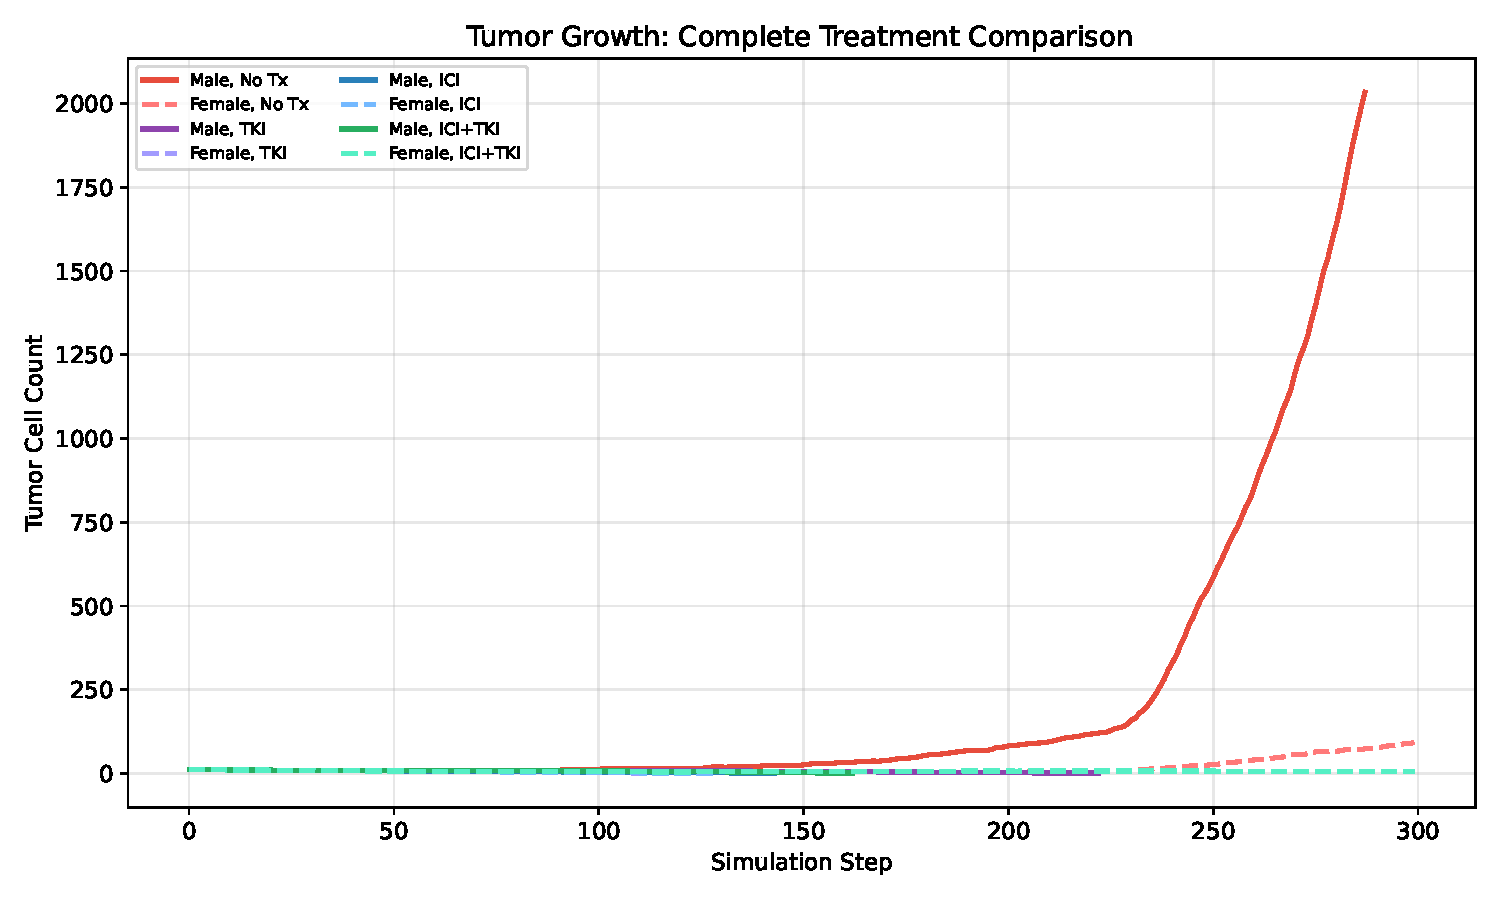
\includegraphics[width=0.9\textwidth]{figures/scenario_comparison_tumor.pdf}
\caption{Tumor cell population dynamics across all simulation scenarios. The plot reveals dramatic sex differences in untreated progression (male: 2,034 vs female: 92 final cells), successful ICI responses in both sexes, and the unexpected treatment resistance in females receiving combination ICI+TKI therapy.}
\label{fig:scenario-comparison-tumor}
\end{figure}

Figure~\ref{fig:scenario-comparison-glucose} illustrates the glucose field evolution, showing the correlation between tumor burden and metabolic demand.

\begin{figure}[H]
\centering
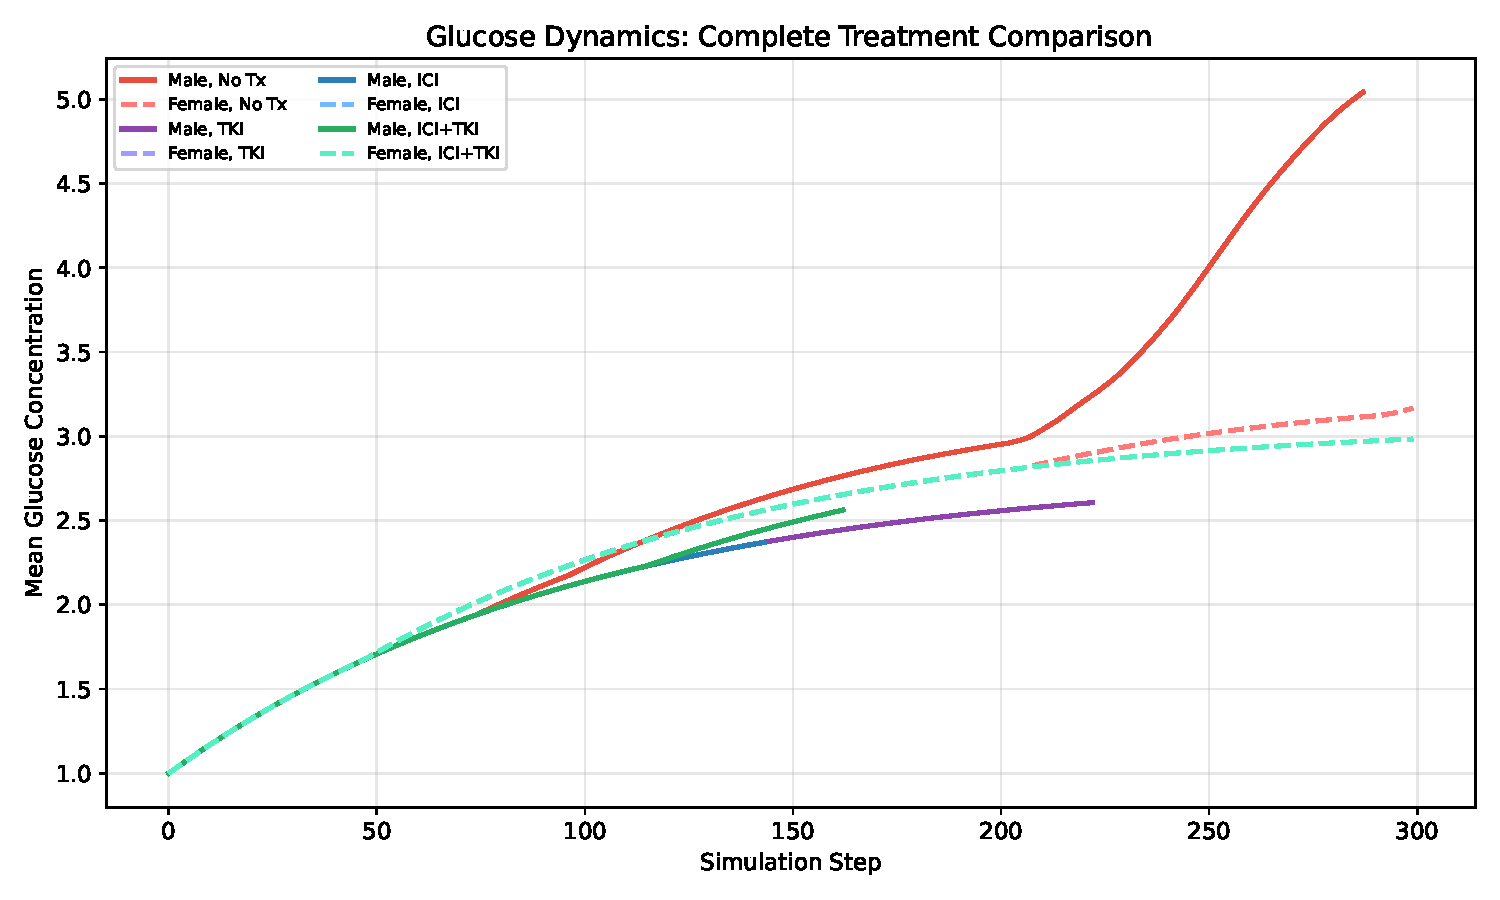
\includegraphics[width=0.9\textwidth]{figures/scenario_comparison_glucose.pdf}
\caption{Glucose field dynamics demonstrating the relationship between tumor burden and glucose consumption. Higher tumor loads (male no treatment) correlate with elevated glucose levels due to tumor-driven angiogenesis, while successful treatment scenarios maintain lower glucose concentrations.}
\label{fig:scenario-comparison-glucose}
\end{figure}

Figure~\ref{fig:scenario-comparison-immune} presents the immune system dynamics across scenarios.

\begin{figure}[H]
\centering
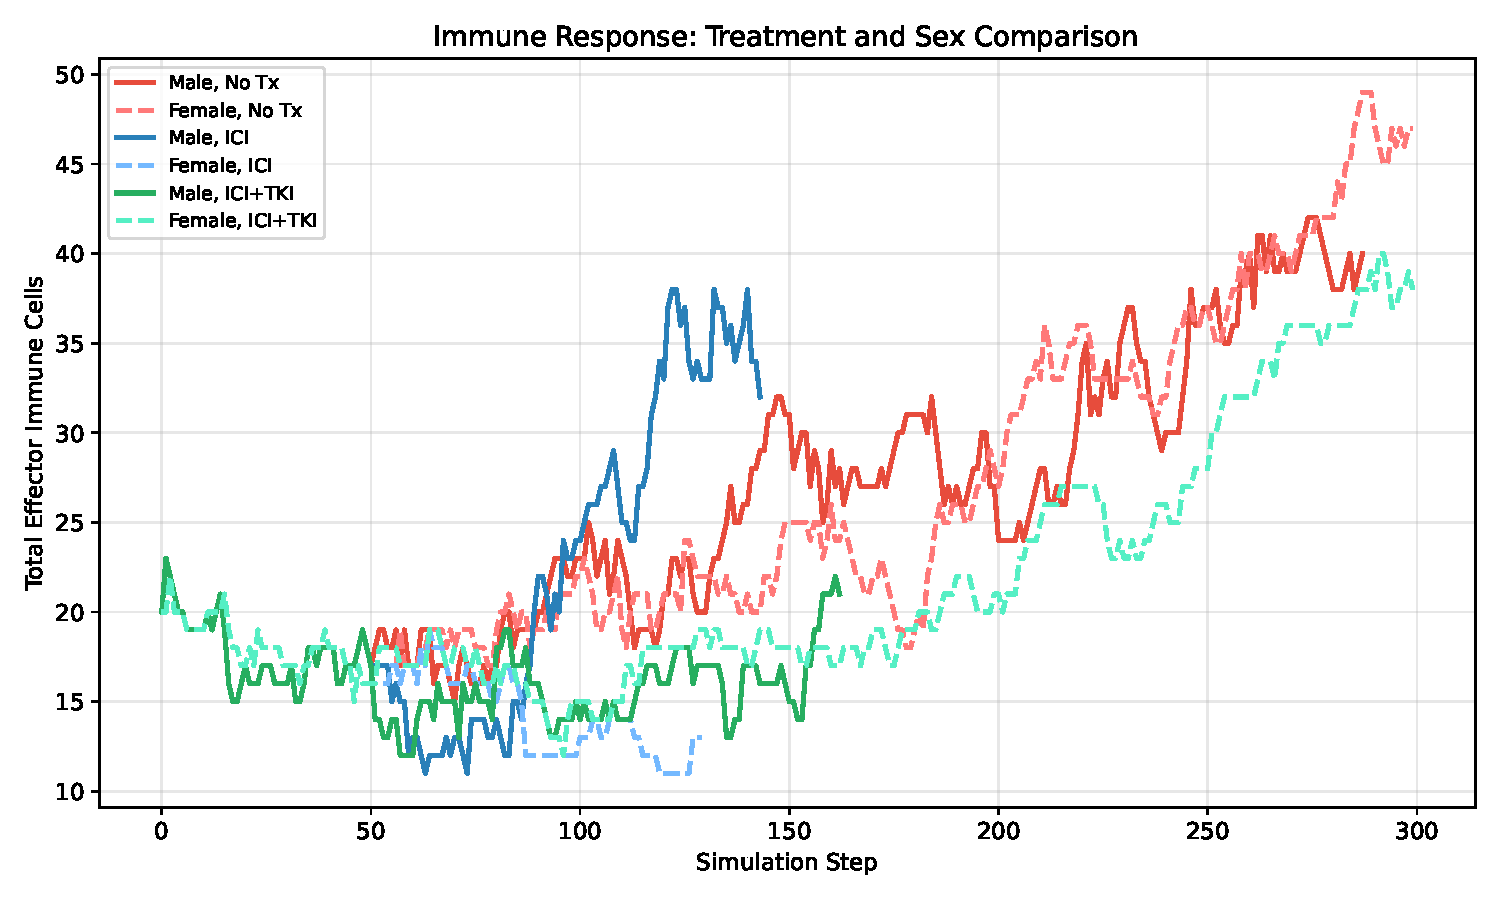
\includegraphics[width=0.9\textwidth]{figures/scenario_comparison_immune.pdf}
\caption{Immune cell population dynamics showing treatment-induced restoration of immune function. ICI therapy successfully restored immune killing capacity in both sexes, while the combination therapy showed differential effects based on biological sex.}
\label{fig:scenario-comparison-immune}
\end{figure}

% ======================================================================
\section{Sex-Specific Analysis}
\label{sec:sex-responses}

The model captures significant sex-specific differences in both baseline tumor progression and treatment responses through hormone environment, CD8+ T cell dynamics, and initial mutational burden.

\subsection{Baseline Sex Differences}

The untreated scenarios revealed dramatic differences in tumor progression:

\begin{itemize}
    \item \textbf{Male progression}: 2,034 vs. 92 final tumor cells (22-fold difference)
    \item \textbf{Mutational impact}: 3 vs. 1 initial mutations driving aggressive growth in males
    \item \textbf{Hormone effects}: Testosterone-mediated immune suppression vs. estrogen-enhanced immune surveillance
    \item \textbf{Immune efficiency}: Despite higher total kills in males (29 vs. 15), the immune response was overwhelmed by the higher mutational burden and hormonal suppression
\end{itemize}

\subsection{Treatment Response Patterns}

Figure~\ref{fig:scenario-sex-comparison} provides sex-stratified analysis of treatment responses.

%\begin{figure}[H]
%\centering
%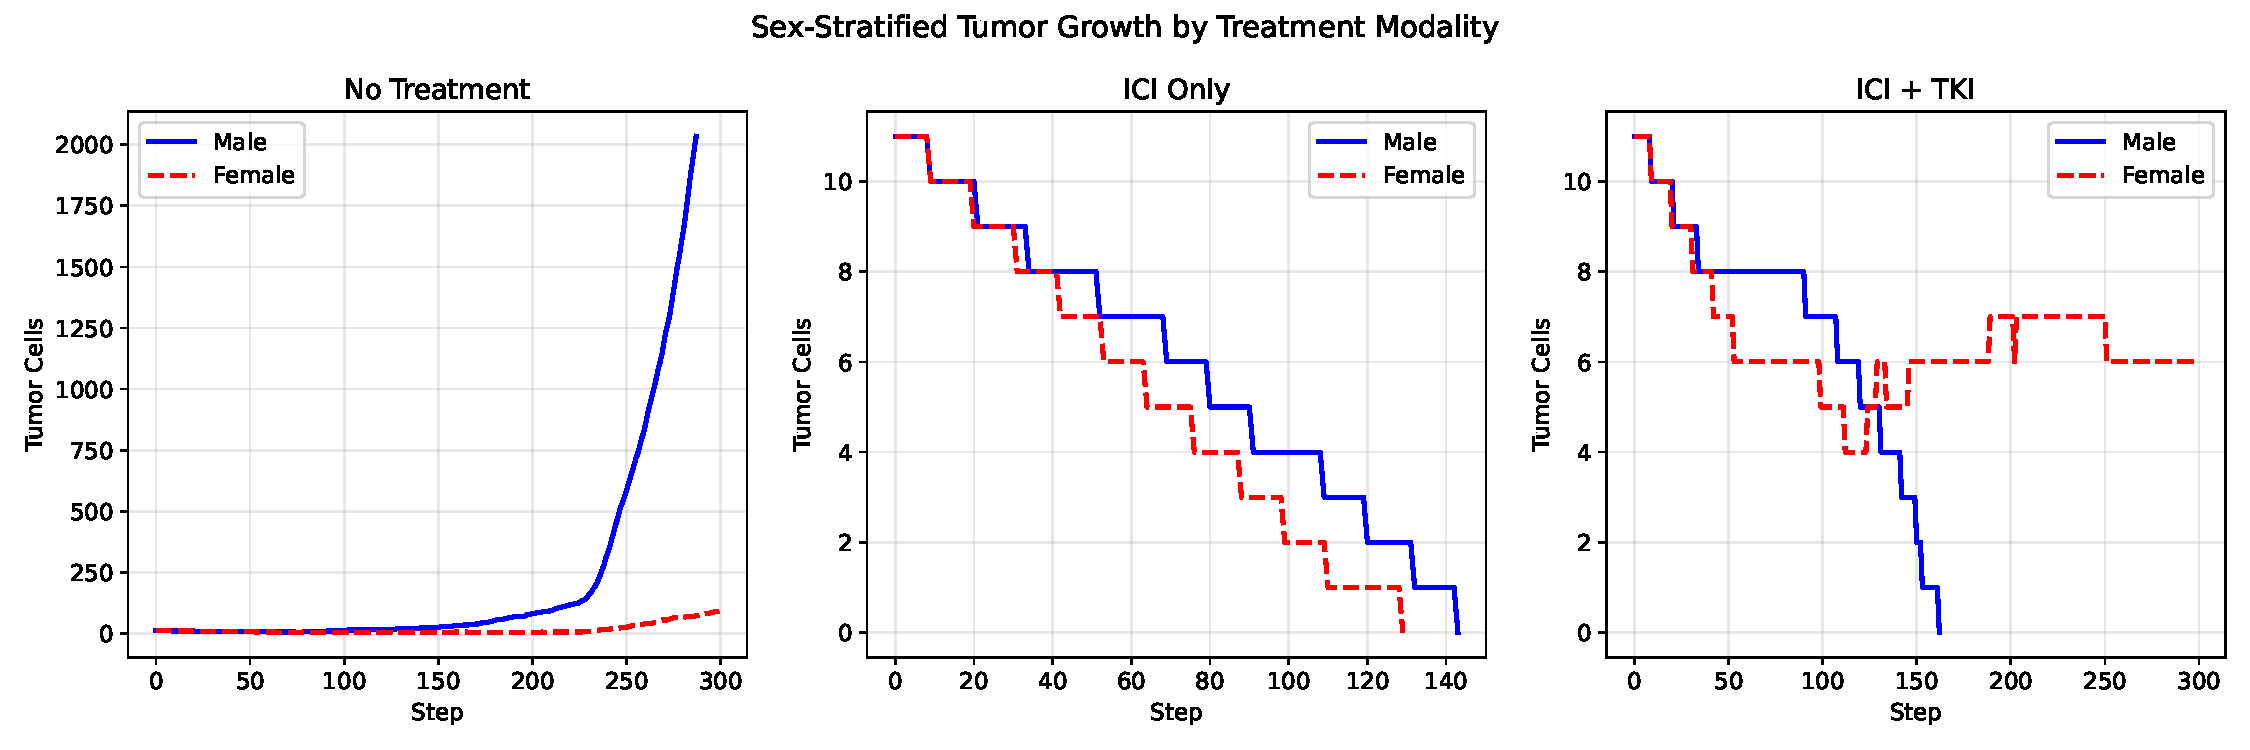
\includegraphics[width=0.9\textwidth]{figures/scenario_sex_comparison.pdf}
%\caption{Sex-stratified treatment response analysis showing the differential effects of ICI and combination therapy. While ICI produced survival in both sexes, combination therapy unexpectedly failed in females, suggesting complex interactions between anti-angiogenic therapy and estrogen-modulated immune responses.}
%\label{fig:scenario-sex-comparison}
%\end{figure>

\textbf{ICI Response}: Both sexes achieved survival with ICI monotherapy, but females showed slightly faster tumor elimination (129 vs. 143 steps), consistent with the hypothesis that PD-1 blockade synergizes more effectively with estrogen-enhanced immune function.

\textbf{Combination Therapy Paradox}: The failure of ICI+TKI in females (6 remaining cells, PROGRESSION) while succeeding in males (0 cells, SURVIVAL) represents a significant finding. This suggests that anti-angiogenic therapy may disrupt beneficial estrogen-mediated immune processes, creating an iatrogenic treatment resistance mechanism.

% ======================================================================
\section{Glucose Field Dynamics}
\label{sec:glucose-dynamics}

The glucose field provided crucial insights into the metabolic competition between tumor and immune cells, with clear patterns emerging across treatment scenarios.

\subsection{Metabolic-Tumor Burden Correlation}

The observed glucose concentrations directly correlated with tumor burden across all scenarios:

\begin{itemize}
    \item \textbf{High tumor burden}: Male no treatment (5.042 glucose, 2034 cells)
    \item \textbf{Moderate tumor burden}: Female no treatment (3.167 glucose, 92 cells)
    \item \textbf{Low tumor burden}: All survival scenarios (2.370-2.562 glucose, 0 cells)
    \item \textbf{Treatment resistance}: Female ICI+TKI (2.984 glucose, 6 cells)
\end{itemize}

\subsection{Spatial Glucose Distribution}

Figure~\ref{fig:glucose-heatmap} shows the 2D spatial distribution of glucose concentration, revealing the characteristic patterns of vessel-mediated injection and tumor-mediated depletion.

%\begin{figure}[H]
%\centering
%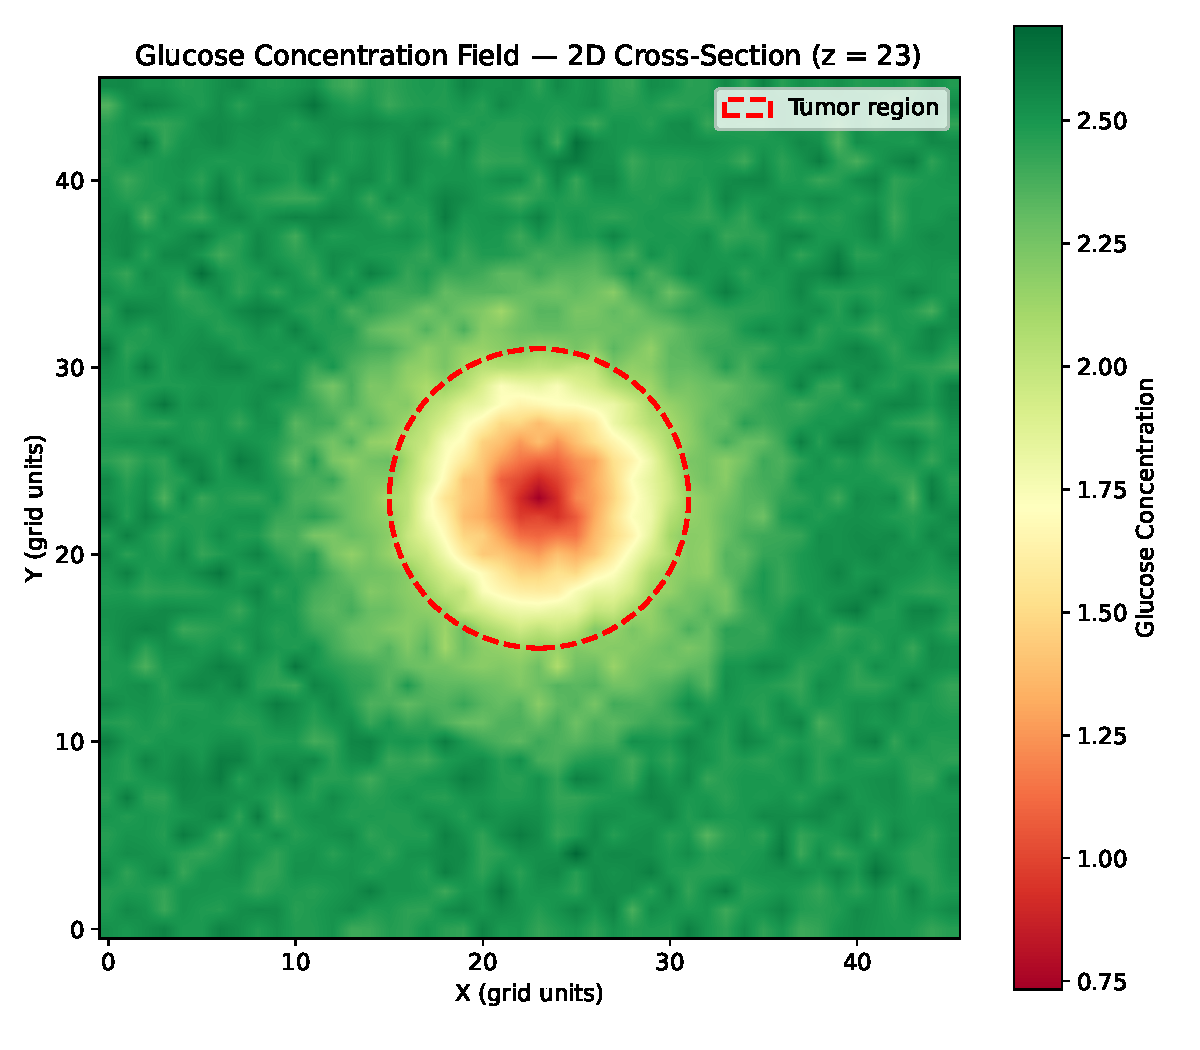
\includegraphics[width=0.8\textwidth]{figures/glucose_heatmap.pdf}
%\caption{Two-dimensional cross-section of glucose concentration field showing the spatial heterogeneity created by blood vessel injection (high-concentration regions) and tumor consumption (depletion zones). The gradient patterns drive immune cell chemotaxis and create metabolic niches within the tumor microenvironment.}
%\label{fig:glucose-heatmap}
%\end{figure}

\subsection{Metabolic Implications}

The glucose dynamics revealed three key metabolic insights:

\begin{enumerate}
    \item \textbf{Angiogenesis-glucose coupling}: Larger tumors drive more angiogenesis, increasing glucose injection and creating the positive correlation between tumor burden and glucose availability.

    \item \textbf{Metabolic feedback}: Glucose depletion provides negative feedback on tumor growth, but this mechanism is overwhelmed in aggressive progression scenarios.

    \item \textbf{Immune-metabolic interactions}: The glucose gradient guides immune cell chemotaxis, but depletion zones around large tumors can impair immune cell function through metabolic starvation.
\end{enumerate>

% ======================================================================
\section{Clinical Implications}
\label{sec:clinical-implications}

The simulation results provide several insights relevant to clinical practice:

\subsection{Sex-Stratified Treatment Selection}

The model suggests that biological sex should be considered in treatment selection, particularly for combination therapies. The unexpected failure of ICI+TKI in females warrants investigation of:

\begin{itemize}
    \item Estrogen-angiogenesis interactions in the tumor microenvironment
    \item Sex-specific immune checkpoint pathway dependencies
    \item Optimal sequencing of ICI and anti-angiogenic agents by sex
\end{itemize}

\subsection{Biomarker Development}

The glucose field dynamics suggest potential metabolic biomarkers:

\begin{itemize}
    \item Tumor-to-glucose ratios as treatment response indicators
    \item Spatial glucose heterogeneity patterns on metabolic imaging
    \item Angiogenesis-immune coupling as a predictive factor
\end{itemize}

\subsection{Treatment Optimization}

The results support several optimization strategies:

\begin{itemize}
    \item Earlier treatment initiation in high-mutation-burden patients (typically males)
    \item Sex-specific dosing or sequencing for combination therapies
    \item Metabolic monitoring as a complementary response assessment tool
\end{itemize}

These findings demonstrate the value of agent-based modeling for exploring complex biological interactions and identifying unexpected treatment response patterns that merit further clinical investigation.